\documentclass[10pt]{article}

\usepackage{amsmath, amsthm, amssymb, amsfonts}
\usepackage{thmtools}
\usepackage{graphicx}
\usepackage{setspace}
\usepackage{geometry}
\usepackage{float}
\usepackage{hyperref}
\usepackage[utf8]{inputenc}
\usepackage[english]{babel}
\usepackage{framed}
\usepackage[dvipsnames]{xcolor}
\usepackage{tcolorbox}
\usepackage{mdframed}
\usepackage{tikz}
\usetikzlibrary{shapes, arrows, positioning}
\usepackage{enumerate}

\newcommand{\E}{\mathbb{E}}
\newcommand{\PP}{\mathbb{P}}

\newcommand{\independent}{\perp\mkern-9.5mu\perp}
\newcommand{\notindependent}{\centernot{\independent}}

\begin{document}


\begin{enumerate}

\item Data from treatment variable $A$, outcome variable $Y$, and scalar covariate $X$ is provided for sample sizes $n\in\{1000,2000,5000,10000,20000\}$. Split the data into two equally sized folds. Estimate the nuisance functions (i.e., the OR function and the propensity score) on one fold, and using the fitted nuisance functions, estimate the average treatment effect on the second fold. 

Report your point estimates and $95\%$ (nonparametric) bootstrap confidence intervals. Present your results both in a table and using boxplots for all sample sizes. Compare the following approaches and make a conclusion regarding the results.
\begin{enumerate}[(a)]
\item OR with linear regression with regressors $(1,A,X)$ (i.e., no interaction term)
\item OR with linear regression with regressors $(1,A,X,AX)$ (i.e., with interaction term)
\item OR with linear regression with regressors $(1,X,X^2,X^3)$ two separate regression on treatment and control groups
\item OR with linear regression with regressors $(1,X,X^2,...,X^6)$ two separate regression on treatment and control groups
\item Same as Part (d), but with imputation OR Estimator
\item Same as Part (d), but with propensity score as the covariate. Use logistic regression with order 2 polynomial for estimating the proensity score
\item IPW with logistic regression with order 1 polynomial
\item IPW with logistic regression with order 2 polynomial
\item Same as Part (h), but with Hajek estimator
\end{enumerate}

\begin{verbatim}

I could not insert an my graphs into the latex but they are in my code. 

\end{verbatim}


\item Give an example such that the weak conditional exchangeability holds but the strong conditional exchangeability does not hold.

Weak conditional exchangeability: $Y^{(a)}\independent A\mid X$ for $a\in\{0,1\}$

Strong conditional exchangeability: $\{Y^{(0)},Y^{(1)}\}\independent A\mid X$

\begin{verbatim}
I'm sorry, I genuinely could not figure this out. Is it even possible?
\end{verbatim}



\item Consider the graphical model below.
\begin{enumerate}[(a)]
\item List all the paths between $A$ and $Y$

\begin{verbatim}
1.) A <- X1 -> Y
2. ) A -> X3 -> Y
3.) A -> X3 <- X2 -> Y
4.) A -> X4 <- Y
5.) A -> X5 <- X4 <- Y
\end{verbatim}

\item For each of the 32 subsets of $\{X_1,X_2,X_3,X_4,X_5\}$, explain which paths are blocked by that subset

\begin{verbatim}
*path numbers defined above
{0}- 2,4,5
{X1}- 2,3,4,5
{X2}- 2,4,5
{X3}- 1,4,5
{X4}- 2,5
{X5}- 2,4
{X1,X2}- 2,3,4,5
{X1,X3}- 1,4,5
{X1,X4}- 2,5
{X1,X5}- 2,3,4
{X2,X3}- 1,2,4,5
{X2,X4}- 2,5
{X2,X5}- 2,4
{X3,X4}- 1,5
{X3,X5}- 1,4
{X4, X5}- 2,5
{X1,X2,X3}- 1,2,3,4,5
{X1,X2,X4}- 2,3,5
{X1,X2,X5}- 2,3,4
{X1,X3,X5}- 1,3,4
{X1,X4,X5}- 2,3,5
{X2,X3,X4}- 1,2,5
{X2,X3,X5}- 1,2,4
{X2,X4,X5}- 2,5
{X3,X4,X5}- 1,5
{X1,X2,X3,X4}- 1,2,3,5
{X1,X2,X3,X5}- 1,2,3,4
{X1,X2,X4,X5}- 2,3,5
{X1,X3,X4,X5}- 1,3,5
{X2,X3,X4,X5}- 1,2,5
\end{verbatim}


\item In order to identify the parameter $\E[Y^{(a)}]$, what variables do we need to adjust for?
\begin{verbatim}
{X1,X2}
{X1}
{X1,X2,X3}

\end{enumerate}

\begin{center}
\tikzstyle{block} = [draw, circle, inner sep=2.5pt, fill=lightgray]
\tikzstyle{input} = [coordinate]
\tikzstyle{output} = [coordinate]
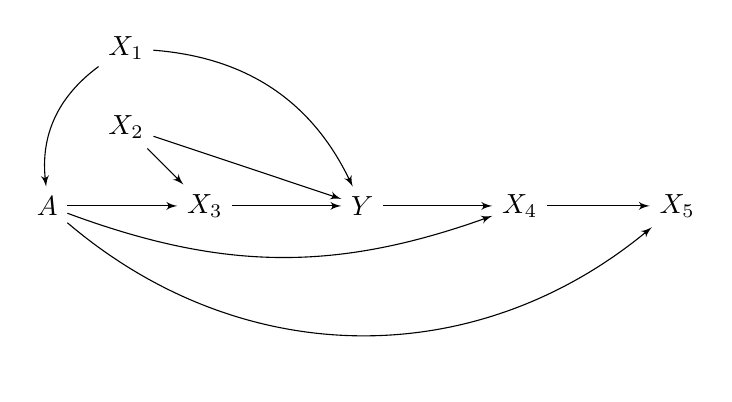
\begin{tikzpicture}
\tikzset{edge/.style = {->,> = latex'}}
            % vertices
	\node[] (a) at  (0,0) {$A$};
	\node[] (y) at  (4,0) {$Y$};
	\node[] (x1) at  (1,2) {$X_1$};
	\node[] (x2) at  (1,1) {$X_2$};
	\node[] (x3) at  (2,0) {$X_3$};
	\node[] (x4) at  (6,0) {$X_4$};
	\node[] (x5) at  (8,0) {$X_5$};
            %edges
	\draw[-stealth][edge, bend left=-0] (a) to (x3);                                                       
	\draw[-stealth][edge, bend left=-0] (x3) to (y);			
	\draw[-stealth][edge, bend left=-0] (y) to (x4);
	\draw[-stealth][edge, bend left=-0] (x4) to (x5);
	\draw[-stealth][edge, bend left=-20] (a) to (x4);
	\draw[-stealth][edge, bend left=-40] (a) to (x5);
	\draw[-stealth][edge, bend left=-0] (x2) to (y);
	\draw[-stealth][edge, bend left=-0] (x2) to (x3);
	\draw[-stealth][edge, bend left=30] (x1) to (y);
	\draw[-stealth][edge, bend left=-30] (x1) to (a);
\end{tikzpicture}
\end{center} 

\item What subsets of $\{X_1,X_2,X_3\}$ can be used to satisfy conditional  
exchangeability in each of the following causal models? What if variables 
$X_1$ and $X_2$ are unobserved, and hence we cannot condition on them? 

\begin{verbatim}
For the first system, the subsets that satisfy conditional exchangeability are:
{0},{X1},{X2},{X1,X2},{X1,X3},{X2,X3}, {X1,X2,X3}. If the X1 and X2 are 
unobserved then {0} is the subset that satisfies condtional exchangeability.

For the second system, the subsets that satisfy conditional exchangeability are: 
{X1,X3}, {X2,X3}, {X1,X2,X3}. No subsets satisfy conditional exchangeability
when X1 and X2 are unobserved

\end{verbatim}

\begin{center}
\tikzstyle{block} = [draw, circle, inner sep=2.5pt, fill=lightgray]
\tikzstyle{input} = [coordinate]
\tikzstyle{output} = [coordinate]
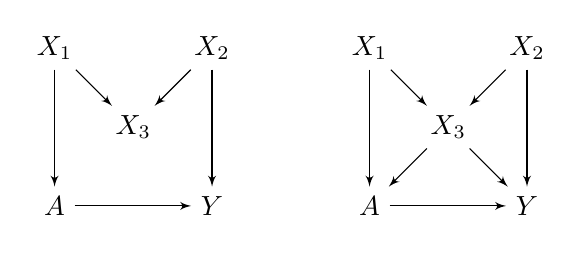
\begin{tikzpicture}
\tikzset{edge/.style = {->,> = latex'}}
            % vertices
	\node[] (a1) at  (0,0) {$A$};
	\node[] (y1) at  (2,0) {$Y$};
	\node[] (a2) at  (4,0) {$A$};
	\node[] (y2) at  (6,0) {$Y$};
	\node[] (x11) at  (0,2) {$X_1$};
	\node[] (x12) at  (1,1) {$X_3$};
	\node[] (x13) at  (2,2) {$X_2$};
	\node[] (x21) at  (4,2) {$X_1$};
	\node[] (x22) at  (5,1) {$X_3$};
	\node[] (x23) at  (6,2) {$X_2$};	
            %edges
	\draw[-stealth][edge, bend left=-0] (x11) to (a1);                                                       
	\draw[-stealth][edge, bend left=-0] (x11) to (x12);
	\draw[-stealth][edge, bend left=-0] (x13) to (x12);
	\draw[-stealth][edge, bend left=-0] (x13) to (y1);
	\draw[-stealth][edge, bend left=-0] (x21) to (a2);                                                       
	\draw[-stealth][edge, bend left=-0] (x21) to (x22);
	\draw[-stealth][edge, bend left=-0] (x23) to (x22);
	\draw[-stealth][edge, bend left=-0] (x23) to (y2);	
	\draw[-stealth][edge, bend left=-0] (x22) to (y2);
	\draw[-stealth][edge, bend left=-0] (x22) to (a2);
	\draw[-stealth][edge, bend left=-0] (a1) to (y1);
	\draw[-stealth][edge, bend left=-0] (a2) to (y2);			
\end{tikzpicture}
\end{center} 

\end{enumerate}



\end{document}